% MACROS:
\newcommand*{\sintheta}[2]{
    \sqrt{\frac{4 m_a^2 (-G_{#1})}{\lambda_{#1} \lambda_{#2}}}
}
\newcommand*{\costheta}[2]{
    \frac{\sqrt{\Lambda_{#1} \Lambda_{#2}} - 2 m_a^2 (t_{#1} + t_{#2} - m_{#2}^2)}{\sqrt{\lambda_{#1}\lambda_{#2}}}
}

%===
% SUBSECTION: A different approach taken from nuclear physics
%===
\subsec{A recursive expression for phase space integrals}
\label{subsec:recursive-relation}
The problem I ran into at the end of \sref{subsec:direct-momentum-integration} was how to use the energy-momentum delta functions to restrict the bounds of integration. 
I spent some time searching the literature for useful references and the most promising were refs.~\cite{James:1968gu,Byckling:1969sx,Isaacson:2021xty}.
\cite{James:1968gu} provides an introduction to Monte Carlo methods and discusses the phase space measure in sec. 9, which covers several ways to deal with the Dirac delta in the phase space integration measure by doing appropriate changes of variables.
The most useful method is covered in sec. 9.6 and is the same one used in \cite{Byckling:1969sx}. 
Ref.~\cite{Byckling:1969sx} extends the treatment in sec. 9.6 of~\cite{James:1968gu} by also introducing momentum transfer variables. 
In this section we will introduce the formalism without momentum transfer variables and cover the case with momentum transfers in \sref{subsec:momentum-transfers}.

Consider the phase space integral $R_n(p_a + p_b)$ defined by
\begin{bluenv}{Phase space integral (without $2 \pi$ factors)}
    \vspace{-3ex}
    \begin{equation}
        \label{eq:phase-space-integral-without-2pi}
        R_n(p_a + p_b) = 
        \int \cdots \int \prod_{i=1}^{n} \delta (p_i^2 - m_i^2) \, \Theta(p_i^0) \, 
        \dd^4 p_i \, \delta^4(p_a + p_b - p_1 - \cdots - p_n).
    \end{equation}
    where $p_i$ now denotes a four-momentum vector in constrast to the previous section where it represented a three-momentum magnitude.
    This is manifestly Lorentz invariant and therefore $R_n$ may only be a function of $s \equiv (p_a + p_b)^2$. 
\end{bluenv}


We note that $R_n(s)$ is related to $\dd \Phi_n(s)$ by
\begin{equation}
    R_n(s) = (2\pi)^{3n - 4} \int  \dd \Phi_n(s) 
    \quad \Rightarrow \quad 
    \int \dd \Phi_3(s) = (2\pi)^{-5} R_3(s).
\end{equation} 


Define the new integration variable $M_{n-1}^2 \equiv (p_a + p_b - p_n)^2$. The physical significance of $M_{n-1}$ is that it is the invariant mass of the first $n-1$ particles, which can be seen using four-momentum conservation: $p_a + p_b - p_n = p_1 + p_2 + \cdots + p_{n-1}$.
It is possible to show that the following recursive relation holds (eqn. (3) of \cite{Byckling:1969sx})
\begin{align}
    \label{eq:recursive-phase-space-relation}
    R_n(s) = 
    \int_{(m_1 + m_2 + \cdots + m_{n-1})^2}^{(\sqrt{s} - m_n)^2} 
    \dd M^2_{n-1} \, \int \dd \Omega_n
    \frac{\sqrt{\lambda(s, M_{n-1}^2, m_n^2)}}{8s} R_{n-1}(M_{n-1}^2)
\end{align}
where $\lambda(x, y, z) = x^2 + y^2 + z^2 - 2 xy - 2 xz - 2yz$ and the solid angle $\dd \Omega_n \equiv \dd \cos \theta_n\, \dd \varphi_n$ defines the direction of $\bm{p}_n$ in the frame where $p_a + p_b = (\sqrt{s}, \bm{0})$. 
\hl{A derivation of {\eref{eq:recursive-phase-space-relation}} can be found in appendix {\ref{app:recursive-relation-derivation}}}.
The upper limit is obtained by requiring that 
\begin{align}
    |\bm{p}_n|^2 = \frac{\lambda(s, M_{n-1}^2, m_n^2)}{4 s} \geq 0\ ,
\end{align}
whereas the lower limit is given by the threshold below which $R_{n-1}(M_{n-1}^2) = 0$.
Both limits can be derived from physical considerations too.
 Repeated application of \eref{eq:recursive-phase-space-relation} yields 
\begin{equation}
\begin{aligned}
    R_n&(s) 
        = 
    \int_{(m_1 + m_2 + \cdots + m_{n-1})^2}^{(\sqrt{s} - m_n)^2}
    \dd M^2_{n-1} \,  \int \dd \Omega_n
    \frac{\sqrt{\lambda(s, M_{n-1}^2, m_n^2)}}{8s} \\
        &\times 
    \int_{(m_1 + m_2 + \cdots + m_{n-2})^2}^{(M_{n-1} - m_{n-1})^2}
    \dd M^2_{n-2}  \, \int \dd \Omega_{n-1}
    \frac{\sqrt{\lambda(M_{n-1}^2, M_{n-2}^2, m_{n-1}^2)}}{8M_{n-1}^2} \\
        &\times \cdots \times
    \int_{(m_1 + m_2)^2}^{(M_3 - m_3)^2}
    \dd M^2_{2}  \, \int \dd \Omega_{3}
    \frac{\sqrt{\lambda(M_{3}^2, M_{2}^2, m_{3}^2)}}{8M_{3}^2} 
    \times 
    \int \dd \Omega_2
    \frac{\sqrt{\lambda(M_{2}^2, m_1^2, m_{2}^2)}}{8M_{2}^2}. 
\end{aligned}
\end{equation}

The important case for me is when $n = 3$:
\begin{bluenv}{Phase space measure for $n = 3$}
    \vspace{-3ex}
    \begin{equation}
        \label{eq:recursive-LIPS-3}
    \begin{aligned}
        R_3(s) &= (2\pi)^{5}\int \dd \Phi_3(s) \\
            &= 
            \int_{(m_1 + m_2)^2}^{(\sqrt{s} - m_3)^2} \dd M_{2}^2 
            \int \dd \Omega_3 \,
            \frac{\sqrt{\lambda (s, M^2_{2}, m_3^2)}}{8s} \,
            \int \dd \Omega_2 \,
            \frac{\sqrt{\lambda (M^2_2, m_1^2, m_2^2)}}{8 M_2^2} \; .
    \end{aligned}
    \end{equation}
\end{bluenv}
It's easy to verify that the number of integration variables matches our expectation of $3(3) - 4 = 5$ since we are integrating over one invariant mass, and two pairs of two angles. 

In the above discussion we have considered $p_a$ and $p_b$ to be fixed.
However, for my purposes I will also be integrating over $p_a$ and $p_b$.
This case seems to be similar to the one considered in~\cite{Isaacson:2021xty} (cf. the example given between their eqs. (12) and (13)).

\begin{figure}[t]
    \centering
    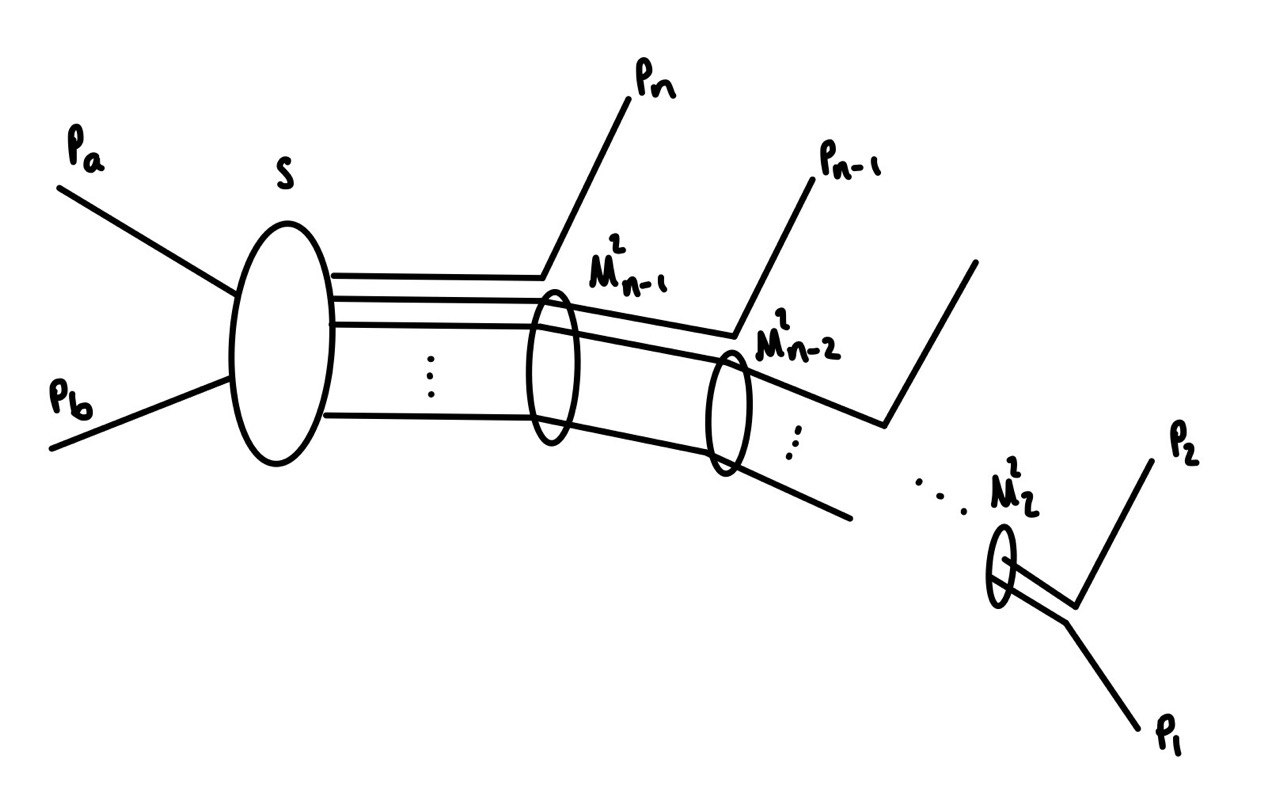
\includegraphics[width=0.6\linewidth]{figs/recursion-diagram.jpg}
    \caption{Illustration of the recursion relation as a sequence of effective $2 \rightarrow 2$ scattering events (this diagram is largely based on pg. 26 of \cite{James:1968gu}).}
    \label{fig:recursion-diagram}
\end{figure}

%====
% SUBSECTION: Writing the integral in terms of momentum transfers 
%====
\subsec{Writing the integral in terms of momentum transfers}
\label{subsec:momentum-transfers}

In sec~\ref{subsec:recursive-relation} we wrote the phase space integral in terms of invariant masses and angles of the three-momenta $\bm{p}_i$ defined in the center-of-mass frame where $\sum_{k=1}^{i} p_k = (M_{i}, \bm{0})$. 
The matrix element in \eref{eq:matrix-element} is a function of the Lorentz invariants $(p_a \cdot p_1), \; (p_b \cdot p_3), \; (p_2 \cdot p_3)$, and $(p_b \cdot p_2) = (- (p_a - p_1 - p_2 - p_3) \cdot p_2)$. 
It is cumbersome to write this matrix element explicitly in terms of the angles $\{ (\theta_i, \varphi_i) : i = 1, 2, \ldots, n\}$ so we would rather use kinematic Lorentz invariants analogous to the Mandelstam variables for $2 \rightarrow 2$ scattering.
To this end it is convenient to \hl{introduce the so-called `momentum transfers' $t_i \equiv Q_i^2 \equiv (p_a - p_1 - \cdots - p_i)^2 = (p_n + p_{n-1} + \cdots + p_{i + 1} - p_b)^2$}.

Some of the dot products (but not all) may be written exclusively in terms of the kinematic variables. For example,
\begin{gather*}
    \begin{align*}
        t_1 &\equiv (p_a - p_1)^2 &&\rightarrow 
            && 2 p_a \cdot p_1 = m_a^2 +  m_1^2 - t_1 \\
        t_2 &\equiv (p_a - (p_1 + p_2))^2 &&\rightarrow 
            && 2 p_a \cdot p_2 = M_2^2 - m_1^2 + t_1 - t_2 \\
        t_3 &\equiv (p_a - (p_1 + p_2 + p_3))^2 &&\rightarrow 
            && 2 p_a \cdot p_3 = t_2 - t_3 - M_2^2 + M_3^2 \\
        M_2^2 &\equiv (p_1 + p_2)^2 &&\rightarrow 
            && 2 p_1 \cdot p_2 = M_2^2 - m_1^2 - m_2^2 \\
        M_3^2 &\equiv (p_1 + p_2 + p_3)^2 &&\rightarrow 
            && 2 (p_1 + p_2) \cdot p_3 = M_3^2 - M_2^2 - m_3^2 \\
        p_b &= p_1 + p_2 + p_3 - p_a &&\rightarrow
            && 2p_b \cdot p_3 = m_3^2 + t_3 - t_2 \\
        & && && 2p_b \cdot p_2 = 2 p_2 \cdot p_3 + m_2^2 + t_2 - t_1
    \end{align*}
\end{gather*}
I could not write $p_2 \cdot p_3$ in terms of the kinematic invariants alone.
This is because we need $3(3) - 4 = 5$ integration variables. Right now we only have $t_1,\ t_2,\ M_2^2$ which is not enough to fully describe the system; two more are required. 
The additional degrees of freedom are given by the azimuthal angles of the $\bm{Q}_i$ vectors $\varphi_1$, $\varphi_2$ as seen in a frame where $p_a = (m_a, \bm{0})$ (cf. \eref{eq:recursive-momentum-transfer-k} which is eq. (14) of~\cite{Byckling:1969sx}.)
It is worth describing in more detail the meaning of the angles $\varphi_1$ and $\varphi_2$. 
I realised on \hl{Aug 18 2023} that these azimuthal angles can't be measured from the same axis. 
The reason for this is the derivation of \eref{eq:recursion-momentum-transfer} and \eref{eq:recursive-momentum-transfer-k} involved a step where we rewrote $\dd^3 Q_{n-1}$ as $\Qmag{n-1}^2 \, \dd \Qmag{n-1} \, \dd \cos \theta_{n-1} \dd \varphi_{n-1}$. 
This transformation requires that $\theta_{n-1}$ be measured from a polar axis and $\varphi_{n-1}$ be measured in the plane perpendicular to that axis.
Since $\theta_{i}$ is defined as the angle between $\Qvec{i}$ and $\Qvec{i+1}$, $\varphi_{i}$ and $\varphi_{i+1}$ can not be measured in the same plane.

To transform $R_n$ into a form in which the momentum transfers appear as variables we must consider the phase space integral as a function of $p_a$ and $-p_b \equiv Q_n$ separately: $R_n = R_n(p_a, Q_n)$. 
Let $Q_i = p_a - p_1 - \cdots - p_i$ so that $p_i = Q_{i-1} - Q_i$. 
Then, \eref{eq:phase-space-integral-without-2pi} becomes
\reversemarginpar\marginnote{In \eref{eq:phase-space-integral-with-momentum-transfer} I didn't write the Heaviside function which picks out positive energies, just pretend it is there so that $(Q_{i-1} - Q_i)^0 > 0$.}
\begin{equation}
    \label{eq:phase-space-integral-with-momentum-transfer}
    \begin{aligned}
        R_n(s) 
        &= \int \bigg[
            \prod_{i=1}^{n}
            \dd^4 Q_i \,
            \delta \big( 
                        (Q_{i-1} - Q_i)^2 - m_i^2
                    \big)
            \bigg] \,
            \delta^4 ( p_a + p_b - \sum_{i=1}^{n} (Q_{i - 1} - Q{i})) \vert_{Q_0 \equiv p_a} \\
        &= \int \bigg[
            \prod_{i=1}^{n}
            \dd^4 Q_i
            \delta \big( 
                        (Q_{i-1} - Q_i)^2 - m_i^2
                    \big)
            \bigg] \,
            \delta^4 ( Q_n + p_b) \\
        &= \int 
            \dd^4 Q_{n-1} 
            \delta \big( 
                        (Q_{n-2} - Q_{n-1})^2 - m_{n-1}^2
                    \big) 
            \bigg[
            \prod_{i=1}^{n-2}
            \dd^4 Q_i
            \delta \big( 
                        (Q_{i-1} - Q_i)^2 - m_i^2
                    \big)
            \bigg] \; .
    \end{aligned}
\end{equation}

The recursion relation is then simply
\begin{equation}
    \label{eq:recursion-momentum-transfer}
    R_n(p_a, Q_n) = \int \dd^4 Q_{n-1} \,
        \delta
        \big(
            (Q_{n-1} - Q_n)^2 - m_n^2    
        \big) \, 
        R_{n-1}(p_a, Q_{n-1}) .
\end{equation}
$R_n$ is now regarded as a function of two invariants $s = s_n = (p_a - Q_n)^2$, and $t_n = Q_n^2$: $R_n = R_n(p_a, Q_n) = R_n(s_n, t_n)$. 
Introducing these variables in \eref{eq:recursion-momentum-transfer} the authors of~\cite{Byckling:1969sx} obtain
\begin{equation}
    \label{eq:recursive-momentum-transfer-s-n}
    R_n(s_n, t_n, s_{n-1}, t_{n-1}) = \int \dd s_{n-1} \, \dd t_{n-1} \, 
        K(s_n, t_n, s_{n-1}, t_{n-1}) \, R_{n-1}(s_{n-1}, t_{n-1}) \, ,
\end{equation}
where
\begin{equation}
    \label{eq:recursive-momentum-transfer-k}
    \begin{aligned}
        K&(s_n, t_n, s_{n-1}, t_{n-1}) \\
        & = \int \dd^4 Q_{n-1} \delta(Q^2_{n-1} - t_{n-1}) \, \delta(s_{n-1} - (p_a - Q_{n-1})^2) \, \delta ( (Q_{n-1} - Q_n)^2 - m_n^2) \\
        & = \int_0^{2\pi} \dd \varphi_{n-1} 
            \frac{1}{4 \sqrt{\lambda(s_n, t_n, m_a^2)}} \, 
            \Theta(- G(t_{n-1}, s_n, s_{n-1}, t_n, m_n^2, m_a^2)) \; ,
    \end{aligned}
\end{equation}
$\Theta(x)$ is the Heaviside step-function, and
$\varphi_{n-1}$ defines the azimuthal angle of $\bm{Q}_{n-1}$ in the frame $p_a = (m_a, \bm{0})$. $G$ is a kinematic function defined by
\begin{equation}
    \begin{aligned}
        \label{eq:G-defn}
        G(x,y,z,u,v,w) & = -\frac{1}{2}
        \begin{vmatrix}
            2 u & x + u - v & u + w - y \\
             & 2x & x - z + w \\
            \text{(symm.)} &  & 2w
        \end{vmatrix} \\
        & = x^2 y + xy^2 + z^2 u + v w^2 + v^2 w \\
        & \phantom{=} + xzw + xuv + yzv + yuw \\
        & \phantom{=} - xy(z + u + v + w) - zu (x + y + v + w) - vw(x + y + z + u) \; .
    \end{aligned}
\end{equation}
In addition, the Dirac deltas impose the following relations hold: 
\begin{bluenv}{Formulas for angles and magnitudes in terms of integration variables}
    \vspace{-2ex}
    \begin{align}
        \Qmag{i} &= \frac{\sqrt{\lambda_i}}{2 m_a} \label{eq:Qmag-formula}\\
        \varepsilon_i &= \frac{\sqrt{\Lambda_i}}{2 m_a} \label{eq:B-epsilon-formula}\\
        \cos \theta_i &\equiv \frac{\Qvec{i}\cdot\Qvec{i+1}}{\Qmag{i}\Qmag{i+1}} 
            =  \frac{\xi_i}{\sqrt{\lambda_i \lambda_{i+1}}} \label{eq:B-costheta-formula}\\
        \sin\theta_i &= \sintheta{i}{i+1} \label{eq:sintheta-formula}
    \end{align}
    where
    \begin{align}
        \label{eq:lambda-definitions}
        \lambda_i &\equiv \lambda(s_i, t_i, m_a^2) \\
        \Lambda_i &\equiv \lambda_i + 4 m_a^2 t_i = (s_i - t_i - m_a^2)^2 \\
        G_i &\equiv G(t_i, s_{i+1}, s_i, t_{i+1}, m_{i+1}^2, m_a^2) < 0 \\
        \label{eq:xi-definition}
        \xi_i &\equiv \sqrt{\Lambda_i \Lambda_{i+1}} - 2 m_a^2 (t_i + t_{i+1} - m_{i+1}^2) \; .
    \end{align}
\end{bluenv}

The main result for this section is the phase space measure for the case of $3$ outgoing particles, which we highlight below.
\begin{bluenv}{$R_n$ for $n = 3$}
    \vspace{-3ex}
    \begin{align}
        \label{eq:recursive-phase-space-with-momentum-transfer-for-n-equal-3}
        R_3(s_3, t_3) 
            = \frac{1}{4\sqrt{\lambda(s_3, t_3, m_a^2)}}
              \int \frac{\dd s_2 \dd t_2 \dd \varphi_2}
                        {4 \sqrt{\lambda(s_2, t_2, m_a^2)}}
              \Theta(- G_2) 
              \int \dd t_1 \dd \varphi_1 \Theta(- G_1)
    \end{align}
    with 
    \begin{gather}
        G_i = G(t_i, s_{i+1}, s_i, t_{i+1}, m_{i+1}^2, m_a^2) \; .
    \end{gather}
\end{bluenv}

To use this method we rewrite parts the integrand by making the replacements:
\begin{align}
    2 p_a \cdot p_1 &\rightarrow m_a^2 +  m_1^2 - t_1 \label{eq:pa-dot-p1-replacement-rule} \\
    2 p_a \cdot p_2 &\rightarrow s_2 - m_1^2 + t_1 - t_2 \\
    2 p_a \cdot p_3 &\rightarrow t_2 - t_3 - s_2 + s_3 \\
    2 p_1 \cdot p_2 &\rightarrow s_2 - m_1^2 - m_2^2 \\
    2p_b \cdot p_3 &\rightarrow m_3^2 + t_3 - t_2 \\
    2p_b \cdot p_2 &\rightarrow 2 p_2 \cdot p_3 + m_2^2 + t_2 - t_1  \ . \label{eq:pb-dot-p2-replacement-rule} 
\end{align}
Then, we will explicitly generate the four-momenta $p_a^{NS}$, $p_b^{NS}$, $p_1^{NS}$, $p_2^{NS}$, $p_3^{NS}$ as seen in the rest frame of the neutron star by 
\begin{enumerate}
    \item Sampling $p_a^{NS}$ and $p_b^{NS}$ from the Fermi-Dirac distribution $f_{FD}(E_a^{NS})$ -- this means that we can drop those factors in the integrand.
    \item Generating the outgoing particle momenta $p_i$ in the frame $p_a = (m_a, 0)$ and then boosting them into a frame where $p_a = p_a^{NS}$ to obtain $p_i^{NS}$.
\end{enumerate}

% ====
% SUBSECTION: Event generation and Monte Carlo integration 
% ====
\subsec{Monte Carlo integration using momentum transfers}
\label{subsec:event-generation}
So far we have rewritten the integral in \eref{eq:emissivity-integral} as 
\begin{align}
    \varepsilon_{3} &= \int f_a f_b (1 - f_1)(1 - f_2) 
                    \, E_3 \sum_{\sigma,\sigma'} |\mathcal{M}|^2 
                    \, \dd \Phi_3 
                    \, \frac{\dd^3 p_a}{(2\pi)^3 2 E_a}
                    \, \frac{\dd^3 p_b}{(2\pi)^3 2 E_b}
\end{align}
where $\dd \Phi_3 = (2\pi)^{-5} R_3$ is given by \eref{eq:recursive-phase-space-with-momentum-transfer-for-n-equal-3} and $\sum_{\sigma, \sigma'} |\mathcal{M}|^2$ is given by \eref{eq:matrix-element} with the replacements given in eqs.~(\ref{eq:pa-dot-p1-replacement-rule})--(\ref{eq:pb-dot-p2-replacement-rule}).
Furthermore, it is understood that the energies that are to be plugged into the $f$ distributions are to be evaluated in the rest-frame of the neutron star. 
Thus, we interpret $\dd^3 p_a$ as $\dd^3 p_a^{NS}$.  
The momenta $p_a^{NS}$ and $p_b^{NS}$ will be sampled in the following way. 
First, rewrite the ingoing momentum integrals
\begin{align}
    \frac{\dd^3 p_a}{2 E_a} &\rightarrow \frac{1}{2}\,\sqrt{E_a^2 - m_a^2} \, \dd E_a \, \dd \cos \theta_a \dd \varphi_a \\
    \frac{\dd^3 p_b}{2 E_b} &\rightarrow \frac{1}{2}\,\sqrt{E_b^2 - m_b^2} \, \dd E_b \, \dd \cos \theta_b \dd \varphi_b\ .
\end{align}
Next, draw $E_a$ and $E_b$ from the distributions $f_a$ and $f_b$. 
This is an example of importance sampling, so the factors of $f_a$ and $f_b$ in the integrand will be canceled out by sampling $E_{a,b}$ in this way.
Sampling can be accomplished by generating realisations of the random variable $X \sim \mathrm{U}(0,1)$ and computing $E_a = F^{-1}(X)$ where $F(E_a) = \frac{1}{N}\int_0^{E_a} f(E) \, \dd E$ is the cumulative distribution function and $N = \int_0^\infty f(E) \, \dd E$ is a normalization factor. 
These integrals can be performed analytically with the results
\begin{bluenv}{Formulas for sampling ingoing particle energies (as seen in the rest-frame of the neutron star)}
    \vspace{-2ex}
    \begin{align}
        N &= \int_0^\infty f(E) \, \dd E = \int_0^\infty \frac{1}{1 + e^{(E-\mu)/T}} \, \dd E = T \ln(1 + e^{\mu / T}) \ , \\
        F(E_a) &= \frac{1}{N} \int_0^{E_a} f(E) \, \dd E = \frac{\ln ( \frac{1 + e^{\mu/T}}{1 + e^{-(E-\mu)/T}})}{\ln(1 + e^{\mu / T})} \ , \\
        F^{-1}(x) &= -T \ln(1 + e^{\mu/T}) \exp{-x \ln(1 + e^{\mu/T}) - 1} + \mu \ .
    \end{align}
\end{bluenv}
I verified these formulas by drawing 100,000 samples of $X$, evaluating $E_a = F^{-1}(X)$ for each, and plotting a histogram of the $E_a$ samples against the distribution $f_a / N$ as shown in \fref{fig:fermi-dirac-sampling}. 
\begin{figure}[htbp]
    \centering
    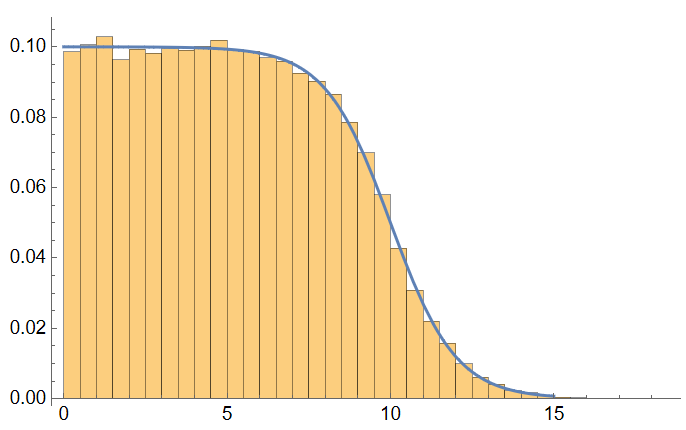
\includegraphics[width=0.7\linewidth]{figs/fd-sampling.png}
    \caption{
        Verification of my method for sampling from a Fermi-Dirac distribution.
        Histogram is on samples obtained using the method described in \sref{subsec:event-generation} and blue curve is $f_{FD}(E)$.
        I chose fiducial values of $\mu = 10$ and $T = 1$. 
    }
    \label{fig:fermi-dirac-sampling}
\end{figure}


\begin{figure}[htbp]
    \centering
    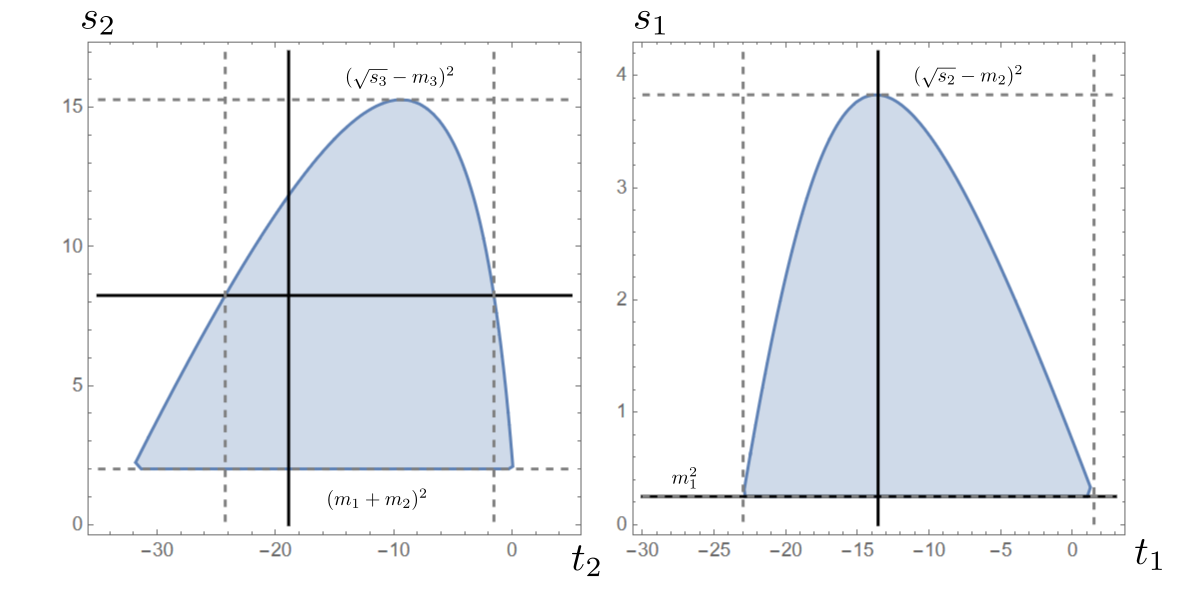
\includegraphics[width=0.9\linewidth]{figs/kinematic-variable-diagram.png}
    \caption{
        Illustration of sampling from the physical region of parameter space dictated by the $\Theta(-G_i)$ step-functions in \eref{eq:recursive-phase-space-with-momentum-transfer-for-n-equal-3}. 
        \emph{(Left:)}
        Region of the $(t_2, s_2)$ plane where $G_2$ is negative (shaded blue).
        This corresponds to the physically allowed region of parameter space.
        The boundary of the region is established by the condition $G_2 = 0$.
        The lower horizontal dashed line is a lower bound established in the case when the C.M. energy of the effective particle $(p_1 + p_2)$ only has enough energy to create the particle with no kinetic energy ($s_2 = (m_1 + m_2)^2$). 
        The upper bound is established when the center of mass energy of $(p_1 + p_2 + p_3)$ creates $p_3$ at rest so that $p_3 = (m_3, 0)$ and the remaining energy is used to create $(p_1 + p_2)$ and supply it with kinetic energy.
        The thick black bars show values of the parameters created using the routine described in the box ``Random number generation for Monte Carlo''.
    }
    \label{<label>}
\end{figure}

\subsubsection{Momentum reconstruction}

To sample $s_i$ we sample a uniform random variable $r_i \sim \mathrm{U}(0,1)$ and compute
\begin{equation}
    \sqrt{s_i} = r_i \left(\sqrt{s_n} - \sum_{j=1}^{n} m_j\right) + \sum_{j=1}^{n} m_j\ .
\end{equation}
Since we are integrating over $s_i$, not $\sqrt{s_i}$, sampling uniformly in $\sqrt{s_i}$ requires us to multiply the integrand by a factor of $2 \sqrt{s_i}$ since $\dd s = \dd (\sqrt{s})^2 = 2 \sqrt{s} \, \dd (\sqrt{s})$.

Next, we take the generated value of $s_i$ (let's call it $\bar{s}_{i}$) and use it to calculate the upper and lower bounds from which we generate $t_i$.
\newline To do this we solve
$G(t_{i}, s_{i+1}, \bar{s}_{i}, t_{i+1}, m_{i+1}^2, m_a^2) = 0$ for $t_{i}$. 
This yields,
\begin{gather}
    \begin{aligned}
        t_{i}^{\pm} 
        =\ 
        &t_{i+1} + m_{i+1}^2 + \\
        &
        \frac{
            (\bar{s}_{i} - s_{i+1} - m_{i+1}^2)(t_{i+1} + s_{i+1} - m_a^2) \pm \sqrt{\lambda(\bar{s}_{i}, s_{i+1}, m_{i+1}^2)\lambda(s_{i+1},t_{i+1},m_a^2)}
        }
        {2\,s_{i+1}} \ .
    \end{aligned} 
\end{gather}
So,
\begin{equation}
    t_i^{\mathrm{gen}} = \gamma_i (t_i^+ - t_i^-) + t_i^-
\end{equation}
where $\gamma_i \sim \mathrm{U}(0,1)$ is another uniform random variable. 
This procedure requires us to weight the generated event by a factor of $(t_i^{+} - t_i^{-})$. Finally, $\varphi_1$ and $\varphi_2$ are sampled independently from $\mathrm{U}(0,2\pi)$.

Once $s_2$, $t_1$, $t_2$, $\varphi_1$, and $\varphi_2$ have been generated using the procedure described above we can reconstruct the outgoing momenta $p_i$ in the following way.
First, calculate the components of $\bm{Q}_i$ in the rest frame of $a$. 
In particular, the components are given by substituting eqs.~(\ref{eq:Qmag-formula}--\ref{eq:xi-definition}) into the following formulas,
\begin{align}
    \bm{Q}_2 &= 
    |\bm{Q}_2|
    ( \sin \theta_2 \cos \varphi_2, \,  
      \sin \theta_2 \sin \varphi_2, \,
      \cos \theta_2) \\
    \bm{Q}_1 &= 
    |\bm{Q}_1| R(\theta_2, \varphi_2)
    ( \sin \theta_1 \cos \varphi_1, \,
      \sin \theta_1 \sin \varphi_1, \,
      \cos \theta_1) 
\end{align}
where $R(\theta_2, \varphi_2)$ is rotation matrix that takes $(0, 0, 1)$ into $(\sin \theta_2 \cos \varphi_2, \sin \theta_2 \sin\varphi_2, \cos \theta_2)$. 
Next, demand calculate the energy-component of $Q_i$ as $Q_i^0 = \pm \sqrt{|\bm{Q}_i|^2 + t_i}$. 
The sign is chosen by imposing the physical momenta have positive energy so, e.g., $(p_2)^0 = (Q_1^0 - Q_2^0) > 0$. 
The way I have implemented this is to first compute the positive sign solutions $\varepsilon_i \equiv \sqrt{|\bm{Q}_i|^2 + t_i}$ and choose $\mathrm{sgn}(Q_i^0) = (-1)^{1 + \Theta(\varepsilon_1 - \varepsilon_2)}$, where $\Theta(x)$ is the Heaviside step function.
The physical momenta are then given in the rest frame of $a$ frame by
\begin{align}
    p_1 &= (p_a - Q_1) \\
    p_2 &= (Q_1 - Q_2) \\
    p_3 &= (Q_2 + p_b) \ .
\end{align}





